% ---------------------------------------------------------------------------------------------------------
\section{Final result: the image-only triage model (the ``69\,\%'' model)}\label{sec:final}

\subsection{Why a triage model}
No model of any family exceeded about 0.57 four-class accuracy on \emph{all} patients
(Sections~\ref{sec:p6}--\ref{sec:bands}). Errors concentrate on ECGs whose echo EF lies near a class limit
(Figure~\ref{fig:boundary}). A model that \emph{answers only when it is confident} and refers the rest to
echocardiography therefore turns the same information into a clinically usable result. The owner chose this framing
(``triage + Mild limitation''). The model was frozen before it was tested.

\subsection{Model definition (frozen 2026-11-06, SHA-256 \texttt{09808d12\ldots})}
\begin{itemize}
  \item \textbf{Input:} the ECG drawing only.
  \begin{itemize}
    \item ECGFounder embedding of the waveform digitised from the PDF;
    \item 118 measurements made on the drawing (clinician-style features);
    \item no printed machine text, no age.
  \end{itemize}
  The patient's sex is used only to place the Normal/Mild cut (52\,\%\ men, 54\,\%\ women), exactly as in the label rule.
  \item \textbf{EF estimate:} the average of a ridge and a LightGBM EF regressor (unverified echo links weighted 0.3).
  \item \textbf{EF grading:} Normal above the sex limit; Mild $45.5$ up to the limit; Moderate $35$--$45.5$; Severe $<35$.
  \item \textbf{Answer rule:} the model answers only when (a) the grade agrees with the image-only four-class
    classifier IMG-C3 (prior rule $\alpha=0.5$), and (b) the EF estimate is at least 3.05 EF points from every cut.
    Otherwise it outputs ``refer to echo''.
  \item \textbf{How the values were chosen:} every threshold was set inside the training folds (nested). The frozen
    copy was refitted on all 837 development ECGs and checked for exact reproduction.
\end{itemize}

\subsection{Results}
\begin{table}[H]\centering\small
\caption{The final image-only model in cross-validation and on the locked test set (scored once,
owner-authorised, 2026-11-06). 95\,\% CIs: corrected repeated-CV (development) and patient-cluster bootstrap (test).}
\label{tab:final}
\begin{adjustbox}{max width=\linewidth}
\begin{tabular}{lcc}\toprule
 & \textbf{Cross-validation} (837 ECGs) & \textbf{Locked test} (199 ECGs) \\\midrule
Triage: share of patients answered & 56\,\% [48, 63] & 49.7\,\% [42.9, 56.7] \\
\textbf{Triage: accuracy on answered patients} & \textbf{0.694} [0.655, 0.736] & \textbf{0.747} [0.660, 0.837] \\
Confident ``Normal'' answers with EF $\ge 41$\,\% & 90\,\% [86, 94] & 85\,\% [77, 92] \\
EF $<41$\,\% patients given a confident ``Normal'' & 15\,\% [8, 22] & 21\,\% [11, 31] \\
Four-class accuracy, all patients (IMG-C3) & 0.558 [0.504, 0.611] & 0.553 [0.485, 0.621] \\
Macro-F1, all patients & 0.441 & 0.453 [0.375, 0.525] \\
Mild precision / recall (all patients) & 0.29 / 0.19 & 0.32 / 0.32 \\\bottomrule
\end{tabular}
\end{adjustbox}
\end{table}

\begin{figure}[H]\centering
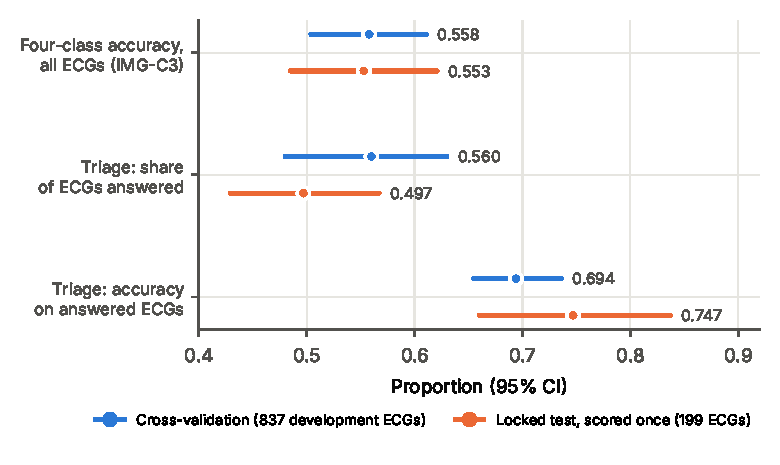
\includegraphics[width=0.78\linewidth]{figures/fig_cv_vs_locked_test.pdf}
\caption{Development estimates carried over to unseen patients: every cross-validation value lies inside its
locked-test confidence interval.}\label{fig:cvtest}
\end{figure}

\begin{figure}[H]\centering
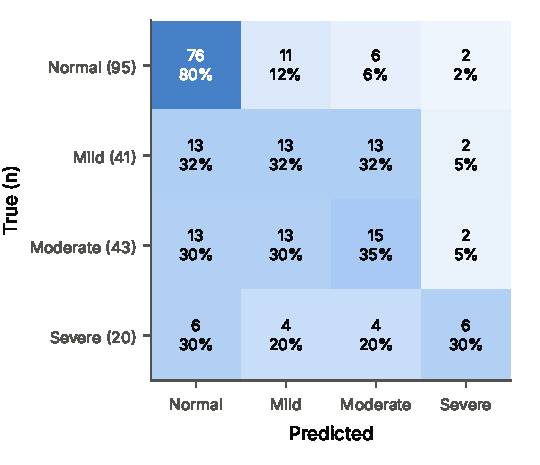
\includegraphics[width=0.5\linewidth]{figures/fig_locked_confusion.pdf}
\caption{Locked-test confusion matrix of the four-class IMG-C3 output (counts and row percentages). Normal is
recognised well; Mild and Moderate are split evenly across Normal, Mild and Moderate.}\label{fig:lockedcm}
\end{figure}

\paragraph{Locked-test details.}
\begin{itemize}
  \item 199 of the 210 locked ECGs form the primary set. 11 were excluded before scoring because their patient key
    forms a near-identical name pair with a development patient.
  \item The 199 ECGs come from 186 patient clusters.
  \item \textbf{Caveat.} The same 210 ECGs had been scored by the original project and in Phase 1 (about 40 models).
    The frozen triage model was developed in Phases 2--7 without any access to them, so the test is independent of its
    development. It is still not a pristine first look at these patients, and a new prospective test set is the
    stronger confirmation.
  \item Triage calls on the locked test: 88 Normal, 10 Moderate, 1 Severe, and no Mild.
  \item Sensitivity analysis on all 210 ECGs: four-class accuracy 0.538; triage 48\,\% answered at 0.743.
\end{itemize}

\subsection{How to state the result}
\begin{quote}
From the ECG image alone, the model gives a confident answer for about half of the patients (56\,\% in
cross-validation, 50\,\% on the locked test), with 0.69--0.75 accuracy on those answers. Most confident answers are
``Normal'', and 85--90\,\% of them exclude moderate or severe LV dysfunction. The remaining patients are referred to
echocardiography. Four-class accuracy on all patients is about 0.55--0.57. Mildly reduced EF cannot be identified
reliably from these printouts.
\end{quote}

\noindent\textbf{Do not claim:}
\begin{itemize}
  \item ``70\,\% accuracy'' without saying \emph{on answered patients} and giving the answered share;
  \item that the triage detects Mild (it made no Mild calls on the locked test);
  \item that it is a stand-alone rule-out: 15--21\,\% of patients with EF $<41$\,\% received a confident ``Normal''.
\end{itemize}
The 210 locked ECGs have now been used, so any further claim needs new ECGs (see the test kit, Appendix~\ref{app:repro}).
